\section{Performance Testing Environment} % (fold)
\label{sec:performance_testing_environment}
To test the framework and applications, we use the following machine specification:
\begin{itemize}
  \item Processor: 2.3 GHz Intel Core i7 (1 processor, 4 cores)
  \item Memory: 8GB 1600 MHz DDR3. 256KB L2 cache per core; 6 MB L3 cache
  \item Graphics: NVIDIA GeForce GT 650M 1024 MB
  \item OS: Mac OS X 10.9.3
  \item Google Chrome version: 35.0.1916.153 (Official Build 274914) 
  \item V8 version: 3.25.28.18
  \item Blink version: 537.36 (@175075)
  \item PPAPI version: 34
\end{itemize}

We use Benchmark JS \cite{benchmarkjs} to easily and accurately measure the amount of time taken to run JavaScript code. Benchmark JS uses high-resolution timers (microsecond precision) and automatically runs the function we wish to test enough times so that it returns statistically significant results. 
% section performance_testing_environment (end)

\section{Application Performance Evaluation} % (fold)
\label{sec:application_performance_evaluation}
\subsection{Bullet Physics Performance} % (fold)
\label{sub:bullet_physics_performance}
The simplest way to measure how well the physics engine performs using Native Calls RPC is to analyse the frames per second (FPS) for a range of scenes of varying complexity. We identify what the biggest impact to the FPS is by measuring how long it takes to make a request and get a response for each frame rendered. We also measure how long it takes to perform the actual simulation step. Finally, we compare these measurements with the original implementation, which was implemented using Native Client Acceleration Modules and tweaked for performance using ArrayBuffers.

\subsubsection{Setup} % (fold)
\label{ssub:bullet_performance_setup}
To test the implementation, we use seven physics scenes. A screenshot of each scene is shown in Figure \ref{fig:bullet_screenshots}. Apart from the Jenga scenes, each scene starts with all the objects falling from the sky and crashing on the ground.

We measure three things - the frame rate, the simulation time, and the round trip time. To measure the frame rate, we simply add to a total of frames requested. A frame is requested by the browser automatically in order to achieve a frame rate of 60 frames per second. This is done using the \lstinline{window.requestAnimationFrame} API, which conveniently takes the computation time for rendering and processing the frame into account. This is why the frame rate drops when the round trip time and simulation time increases. We measure the total simulation time inside the C++ application by taking time stamps between and after the simulation step and calculating the difference. We send it back with the results every time we do the simulation. Finally, we calculate the round trip time by taking timestamps before and after the RPC call and taking a difference. We average all this data over a period of one second and send it to be plotted.

For each second, the average time per frame is calculated. This is the inverse of frames per second, and we call this period the \emph{frame time}. During that time, a RPC request is made and a response is received. We call the period between making a request and receiving a response the \emph{RPC time}. We calculate these times and average them for each second for a period of 20 seconds - the \emph{elapsed time}. Figure \ref{fig:frame-time-vis} shows a visualisation of this terminology.

The graph is plotted in real time in the browser, but we make sure not to use the same \lstinline{window} object - as this will impact JavaScript performance and give us skewed results. Instead, we send the data to be plotted in a different window - which in Chrome corresponds to a different process. HighCharts was chosen to quickly and easily create the realtime graph with very little configuration.

The actual implementation of the RPC library for the physics simulation is discussed in the qualitative evaluation section \ref{sub:implementation_bullet_evaluation} on page \pageref{sub:implementation_bullet_evaluation}.

\begin{figure}
    \centering
    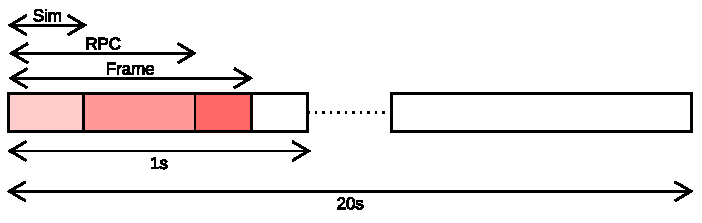
\includegraphics[width=0.7\textwidth]{FrameTimeVisualisation.pdf} 
    \caption{A graphical representation showing the times measured.}
    \label{fig:frame-time-vis}
\end{figure}

\begin{figure}
        \centering
        \begin{subfigure}[b]{0.45\textwidth}
                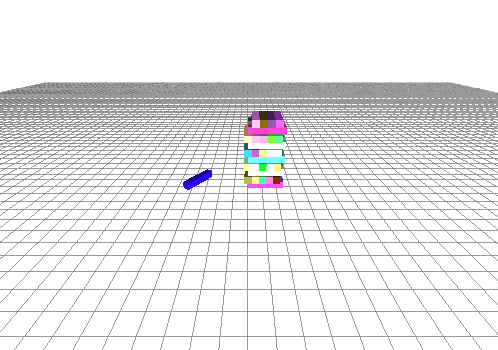
\includegraphics[width=\textwidth]{jenga_10.png}
                \caption{Jenga 10}
                \label{fig:screenshot_jenga_10}
        \end{subfigure}%
        ~ %add desired spacing between images, e. g. ~, \quad, \qquad, \hfill etc.
          %(or a blank line to force the subfigure onto a new line)
        \begin{subfigure}[b]{0.45\textwidth}
                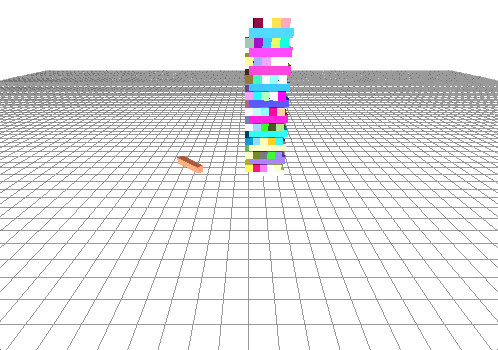
\includegraphics[width=\textwidth]{jenga_20.png}
                \caption{Jenga 20}
                \label{fig:screenshot_jenga_20}
        \end{subfigure}
        ~ %add desired spacing between images, e. g. ~, \quad, \qquad, \hfill etc.
          %(or a blank line to force the subfigure onto a new line)
        \begin{subfigure}[b]{0.45\textwidth}
                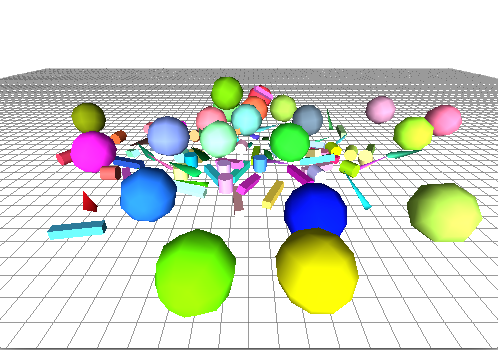
\includegraphics[width=\textwidth]{random_shapes.png}
                \caption{Random Shapes}
                \label{fig:random_shapes}
        \end{subfigure}
        ~ %add desired spacing between images, e. g. ~, \quad, \qquad, \hfill etc.
          %(or a blank line to force the subfigure onto a new line)
        \begin{subfigure}[b]{0.45\textwidth}
                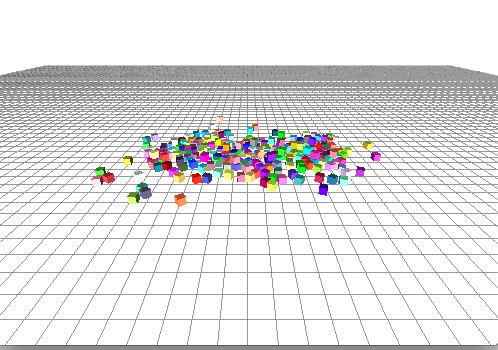
\includegraphics[width=\textwidth]{cubes_250.png}
                \caption{250 Cubes}
                \label{fig:cubes_250}
        \end{subfigure}
        \begin{subfigure}[b]{0.45\textwidth}
                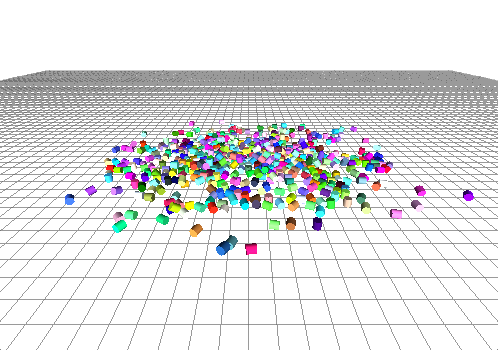
\includegraphics[width=\textwidth]{cylinders_500.png}
                \caption{500 Cylinders}
                \label{fig:cylinders_500}
        \end{subfigure}%
        ~ %add desired spacing between images, e. g. ~, \quad, \qquad, \hfill etc.
          %(or a blank line to force the subfigure onto a new line)
        \begin{subfigure}[b]{0.45\textwidth}
                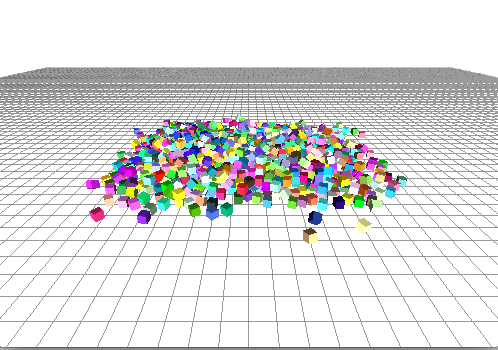
\includegraphics[width=\textwidth]{cubes_1000.png}
                \caption{1000 Cubes}
                \label{fig:cubes_1000}
        \end{subfigure}
        ~ %add desired spacing between images, e. g. ~, \quad, \qquad, \hfill etc.
          %(or a blank line to force the subfigure onto a new line)
        \begin{subfigure}[b]{0.45\textwidth}
                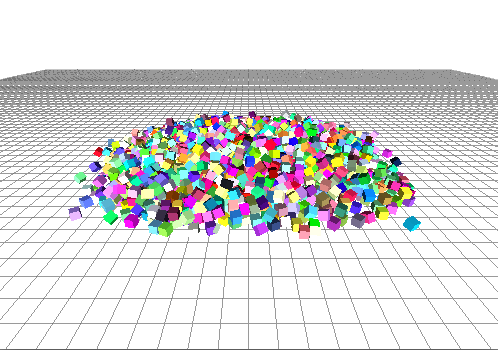
\includegraphics[width=\textwidth]{cubes_2000.png}
                \caption{2000 Cubes}
                \label{fig:cubes_2000}
        \end{subfigure}
        \caption{The bullet physics scenes used in the benchmark}\label{fig:bullet_screenshots}
\end{figure}


% subsubsection bullet_performance_setup (end)

\subsubsection{Results and comparison} % (fold)
\label{ssub:results_bullet_physics_performance}

\begin{table}[h]
    \begin{subtable}[h]{\textwidth}
        \centering
\begin{tabular}{l|lll|lll|lll|lll}
\multirow{3}{*}{Scene} & \multicolumn{9}{l|}{Time / ms}                                                          & \multicolumn{3}{l|}{\multirow{2}{*}{FPS}} \\ \cline{2-10}
                       & \multicolumn{3}{l|}{Frame} & \multicolumn{3}{l|}{RPC} & \multicolumn{3}{l|}{Simulation} & \multicolumn{3}{l|}{}                     \\ \cline{2-13} 
                       & $\mu$     & Max     & Min     & $\mu$     & Max    & Min    & $\mu$       & Max       & Min      & $\mu$          & Max          & Min          \\ \hline
A                      & 17       & 18     & 16     & 17       & 18    & 16    & 0.11       & 0.13     & 0.10    & 60            & 61          & 55          \\
B                      & 17       & 18     & 16     & 17       & 18    & 16    & 0.35       & 2.93     & 0.08    & 60            & 61          & 56          \\
C                      & 17       & 17     & 16     & 17       & 17    & 16    & 0.45       & 0.90     & 0.23    & 60            & 61          & 59          \\
D                      & 17       & 21     & 16     & 17       & 21    & 16    & 0.67       & 1.80     & 0.20    & 59            & 61          & 48          \\
E                      & 21       & 23     & 17     & 21       & 24    & 17    & 2.46       & 5.73     & 1.08    & 49            & 58          & 44          \\
F                      & 39       & 45     & 17     & 38       & 43    & 17    & 10.80      & 14.56    & 0.11    & 25            & 60          & 22          \\
G                      & 72       & 91     & 34     & 73       & 91    & 34    & 23.73      & 41.08    & 0.91    & 14            & 29          & 11         
\end{tabular}
        \caption{Using Native Calls}
    \end{subtable}
    ~
    \begin{subtable}[h]{\textwidth}
        \centering
\begin{tabular}{l|lll|lll|lll|lll}
\multirow{3}{*}{Scene} & \multicolumn{9}{l|}{Time / ms}                                                          & \multicolumn{3}{l|}{\multirow{2}{*}{FPS}} \\ \cline{2-10}
                       & \multicolumn{3}{l|}{Frame} & \multicolumn{3}{l|}{RPC} & \multicolumn{3}{l|}{Simulation} & \multicolumn{3}{l|}{}                     \\ \cline{2-13} 
                       & $\mu$     & Max     & Min     & $\mu$     & Max    & Min    & $\mu$       & Max       & Min      & $\mu$          & Max          & Min          \\ \hline
A                      & 17       & 18     & 16     & 17       & 18    & 16    & 0.13       & 0.14     & 0.12    & 60            & 61          & 55          \\
B                      & 17       & 18     & 16     & 17       & 18    & 16    & 0.38       & 3.37     & 0.10    & 60            & 61          & 57          \\
C                      & 17       & 17     & 16     & 17       & 20    & 16    & 0.60       & 0.93     & 0.27    & 60            & 61          & 59          \\
D                      & 17       & 19     & 16     & 17       & 20    & 17    & 1.14       & 1.87     & 0.22    & 60            & 61          & 52          \\
E                      & 17       & 18     & 16     & 17       & 26    & 16    & 2.64       & 5.82     & 0.97    & 60            & 61          & 55          \\
F                      & 19       & 21     & 17     & 19       & 24    & 17    & 12.06      & 15.49    & 1.09    & 53            & 59          & 48          \\
G                      & 35       & 40     & 17     & 35       & 42    & 18    & 30.77      & 37.93    & 8.86    & 29            & 58          & 25         
\end{tabular}
        \caption{Using NaClAM}
    \end{subtable}
\caption{Time measurements for the bullet physics demo, using different implementations}
\label{table:bullet_performance}
\end{table}


Table \ref{table:bullet_performance} shows the results of the measurements taken during the simulation every second, over a duration of 20 seconds. Figure \ref{fig:bullet_screenshots} shows which scene corresponds to which capital letter (for example, scene `E' is referring to the simulation of 500 cylinders).

Because the simulation is affected by time, the table shows the range of values taken for each measurement.

We can see that scenes A, B, C, D, and E have roughly similar results for both implementations. Scenes F and G show some more interesting results. Figures \ref{fig:bullet_graph_cyl500}, \ref{fig:bullet_graph_cube1000}, and \ref{fig:bullet_graph_cube2000} show some plots showing how the simulation time and frame time change per second for scenes E, F and G respectively, using the Native Calls and NaClAM implementations.

\begin{figure}
        \centering
        \begin{subfigure}[b]{\textwidth}
                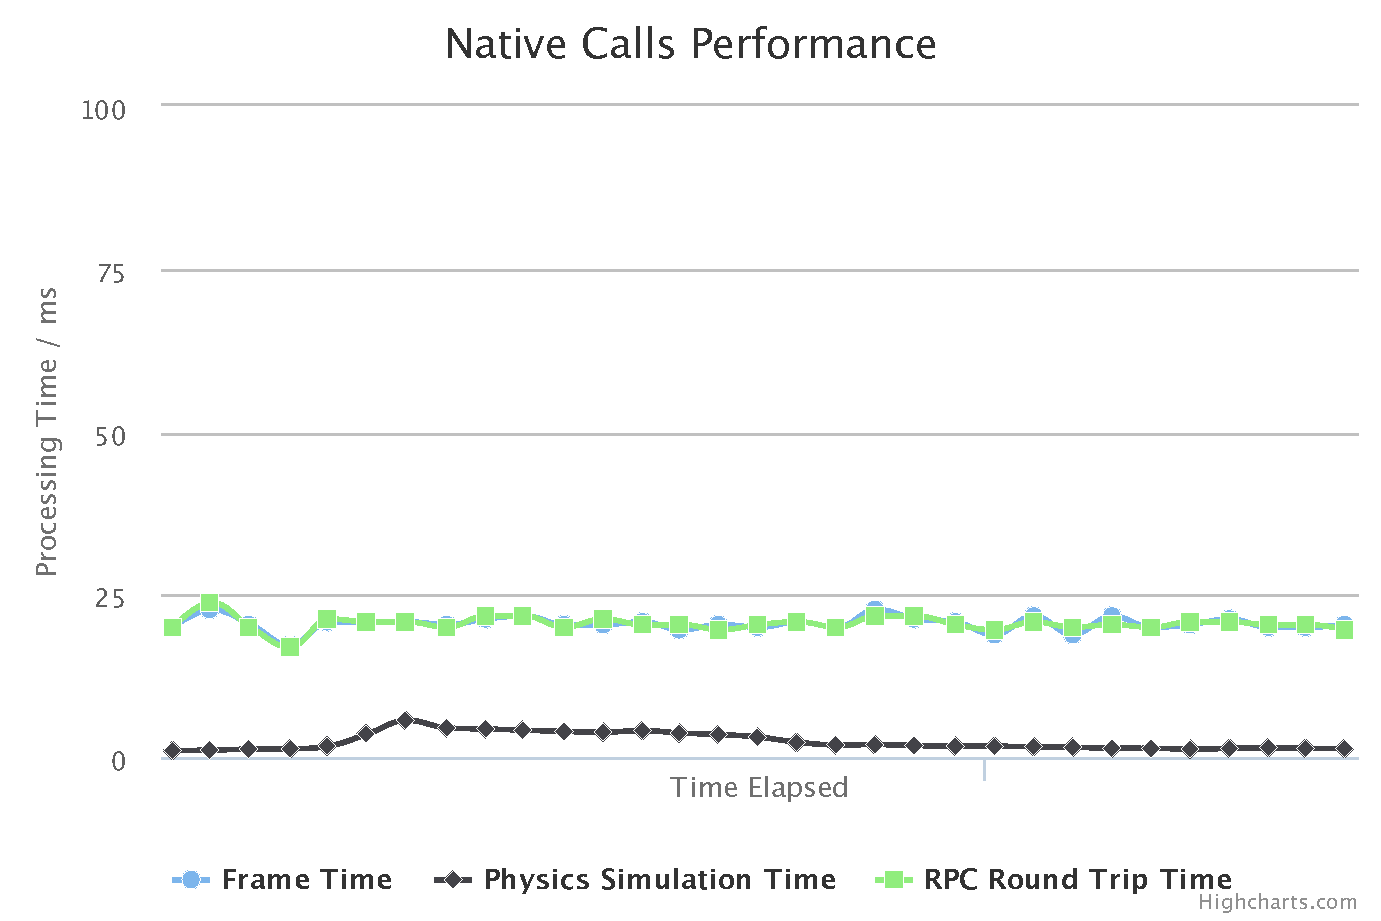
\includegraphics[width=\textwidth]{bulletdata_cylinder500_nc.pdf}
                % \caption{Using Native Calls}
                \label{fig:bulletdata_cylinder500_nc}
        \end{subfigure}%
        \\
        \begin{subfigure}[b]{\textwidth}
                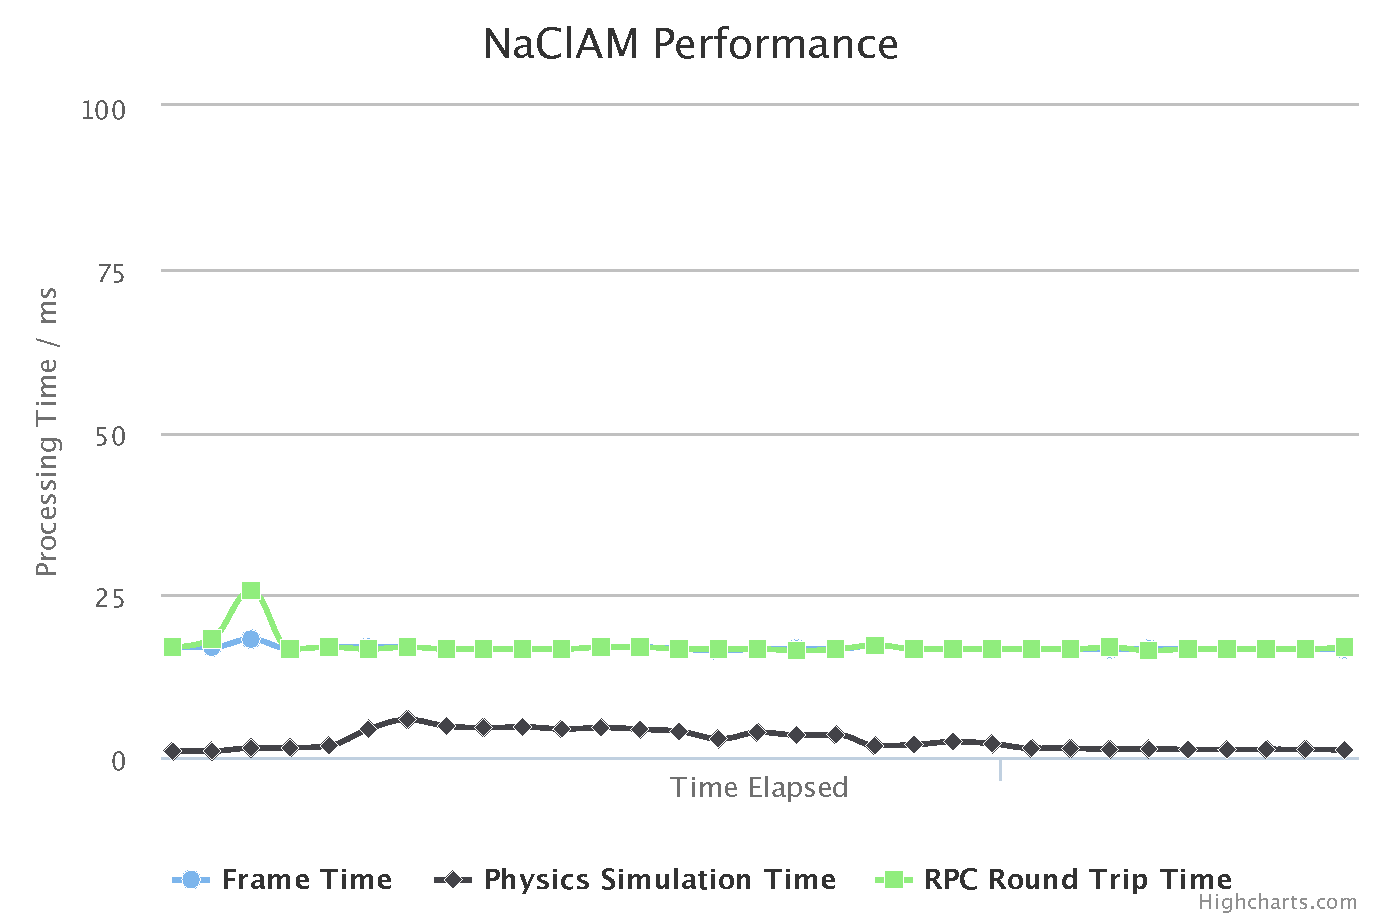
\includegraphics[width=\textwidth]{bulletdata_cylinder500_naclam.pdf}
                % \caption{Using NaClAM}
                \label{fig:bulletdata_cylinder500_naclam}
        \end{subfigure}
        \caption{The mean processing times per second over a period of 20 seconds, for Scene E: 500 cylinders. The two graphs show the results using the same scene but different implementations.}
        \label{fig:bullet_graph_cyl500}
\end{figure}

\begin{figure}
        \centering
        \begin{subfigure}[b]{\textwidth}
                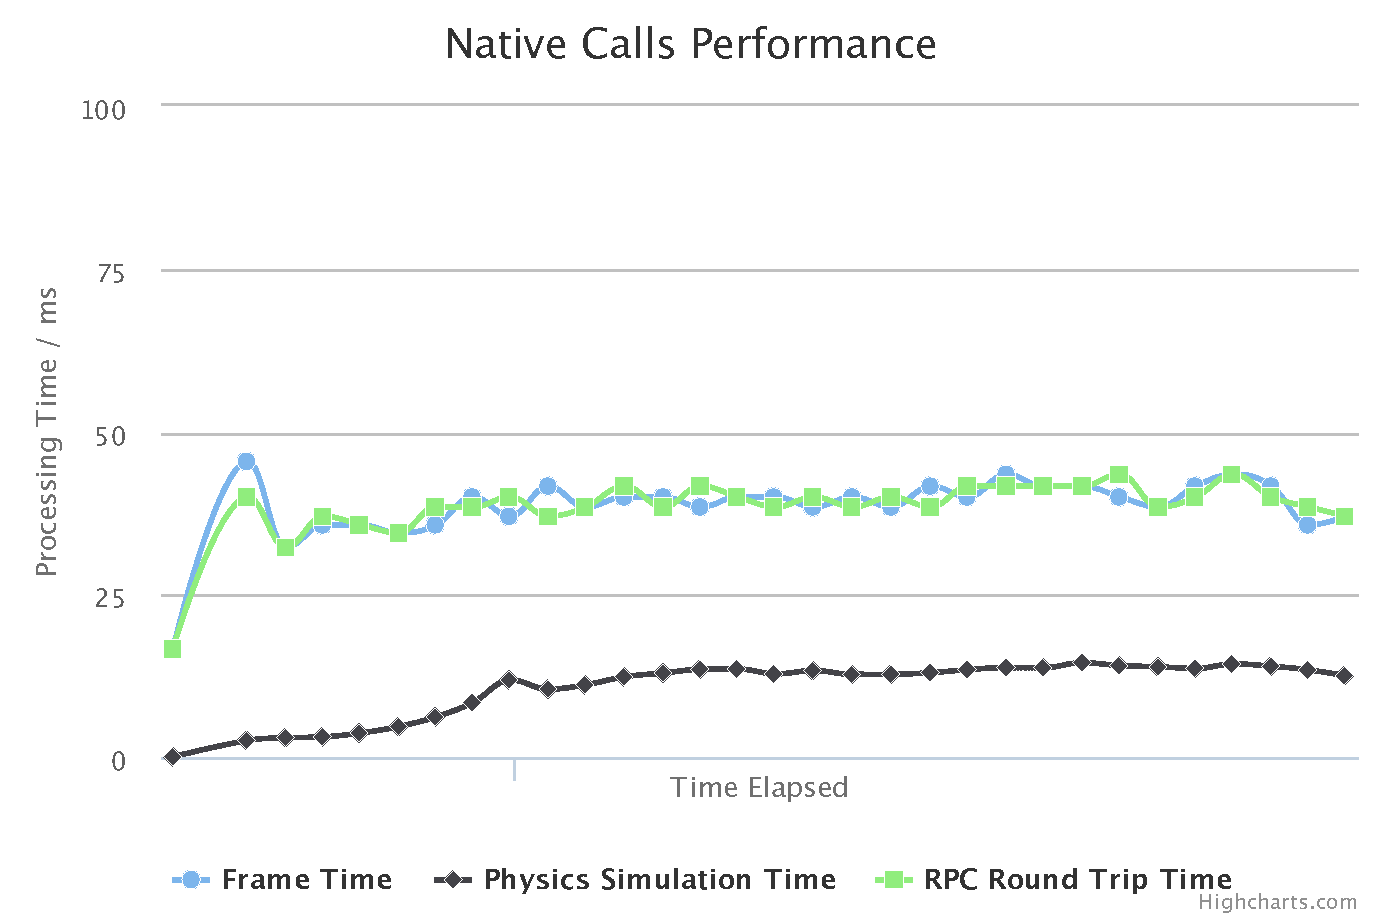
\includegraphics[width=\textwidth]{bulletdata_cube1000_nc.pdf}
                % \caption{Random Shapes}
                % \label{fig:random_shapes}
        \end{subfigure}
        \\
        \begin{subfigure}[b]{\textwidth}
                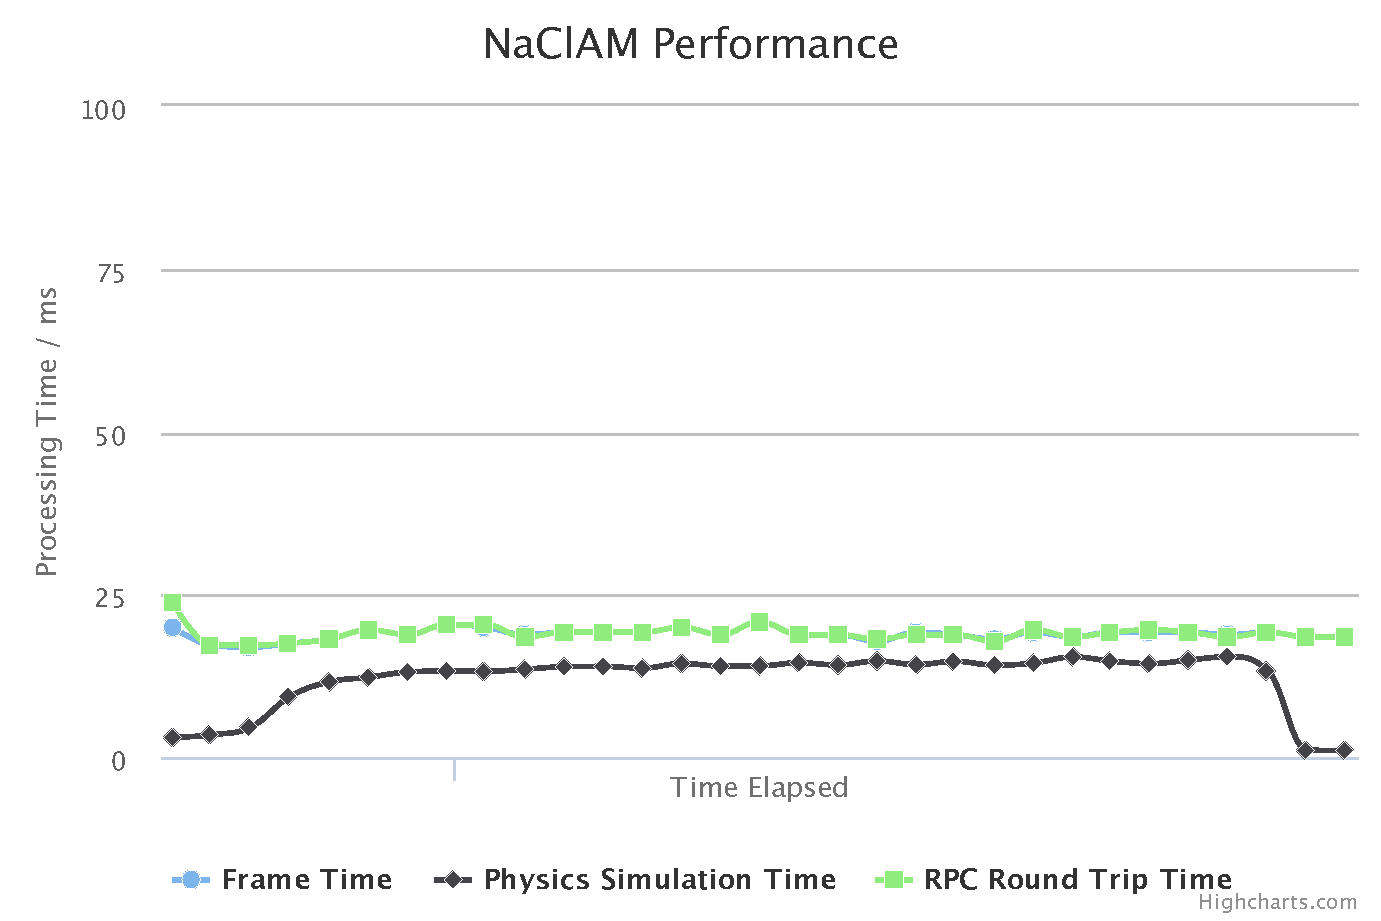
\includegraphics[width=\textwidth]{bulletdata_cube1000_naclam.pdf}
                % \caption{250 Cubes}
                % \label{fig:cubes_250}
        \end{subfigure}
        \caption{The mean processing times per second over a period of 20 seconds, for Scene F: 1000 cubes.}
        \label{fig:bullet_graph_cube1000}
\end{figure}

\begin{figure}
        \centering
        \begin{subfigure}[b]{\textwidth}
                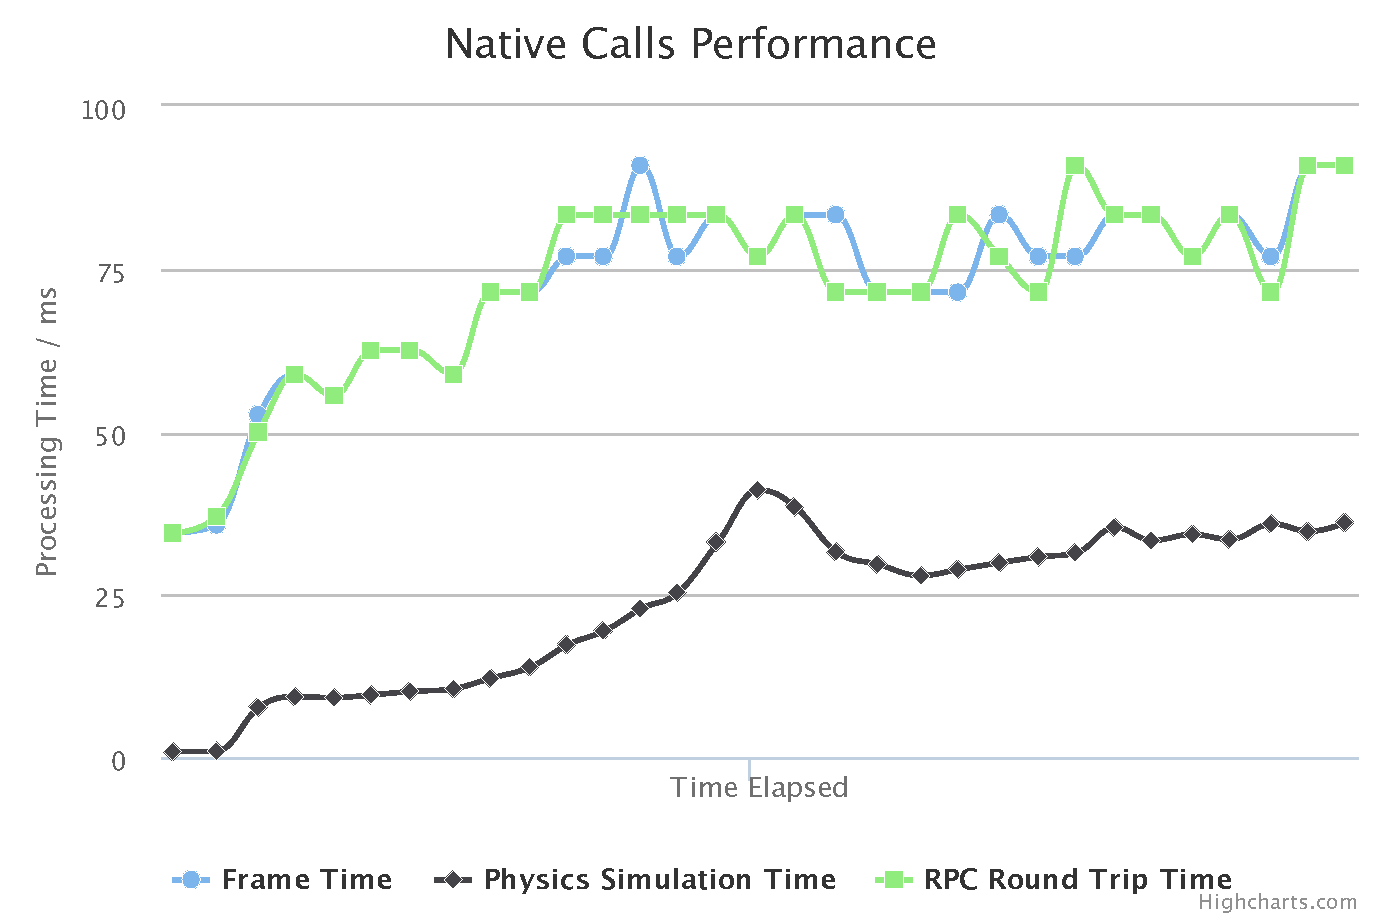
\includegraphics[width=\textwidth]{bulletdata_cube2000_nc.pdf}
                % \caption{500 Cylinders}
                % \label{fig:cylinders_500}
        \end{subfigure}%
        \\
        \begin{subfigure}[b]{\textwidth}
                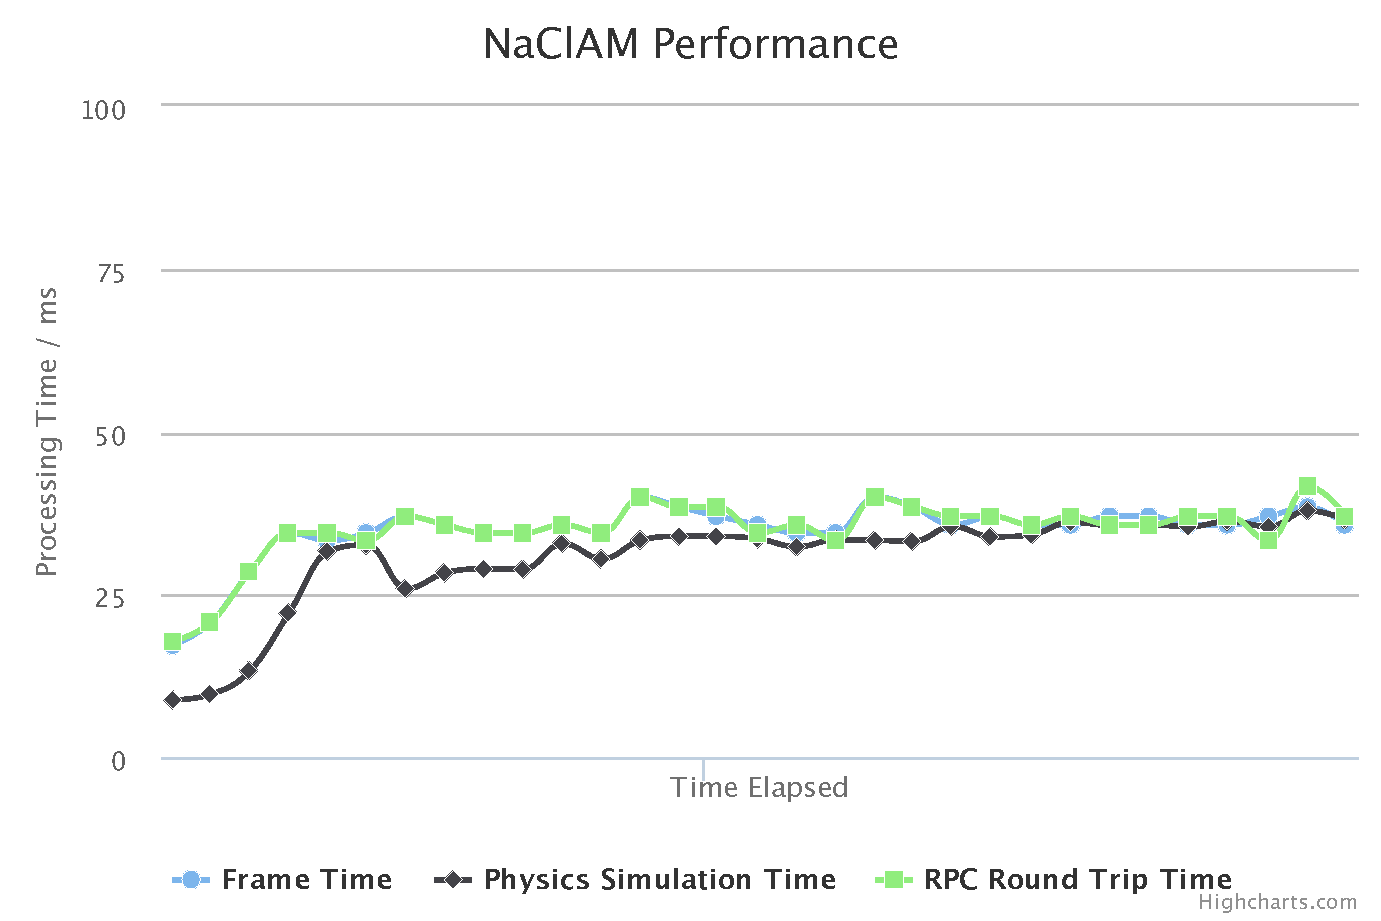
\includegraphics[width=\textwidth]{bulletdata_cube2000_naclam.pdf}
                % \caption{1000 Cubes}
                % \label{fig:cubes_1000}
        \end{subfigure}
        \caption{The mean processing times per second over a period of 20 seconds, for Scene G: 2000 cubes.}
        \label{fig:bullet_graph_cube2000}
\end{figure}

% subsubsection results_bullet_physics_performance (end)

\subsubsection{Analysis} % (fold)
\label{ssub:bullet_physics_performanceanalysis}
From the graphs and tables, we can obviously see how the performance impact of our framework gets higher and higher with more and more objects being sent. We can see how for large scenes such as 2000 cubes, the Native Calls implementation performs almost two times worse than the NaClAM implementation. However for smaller scenes, the two implementations have very similar performance.

From the graphs we can see how the Native Calls framework contributes to the performance impact. For example, in Figure \ref{fig:bullet_graph_cube2000}, the large space between the physics simulation time line and the RPC round trip time line is an indication that the framework is doing most of the processing in the RPC call, not the simulation. When we compare this to the NaClAM version in the same figure, it is clear that most of the processing happens in the physics simulation.

The most likely reason for these two observations is that the data marshalling on the C++ Native Calls RPC framework implementation negatively impacts the performance. In our implementation, the data is processed in O(n) time in order to convert the received \lstinline{pp::VarArray} array of objects into a \lstinline{std::vector} of \lstinline{struct}s. In section \ref{sec:performance_evaluation} (page \pageref{sec:performance_evaluation}), we find that converting WebIDL dictionaries is also quite slow, compared to converting an array of numbers. When we compare this to the NaClAM implementation, we can see that the NaClAM version has almost O(1) time, since the data is only being read and is shared between the module and JavaScript. This is explained in section \ref{sec:naclam} on page \pageref{sec:naclam}.

% subsubsection bullet_physics_performanceanalysis (end)


% subsection bullet_physics_performance (end)

\subsection{Oniguruma Regular Expressions Performance} % (fold)
\label{sub:oniguruma_regular_expressions_performance}
To get an insight of the performance of the oniguruma library for Native Client using Native Calls, we shall count the number of regular expression matches. We compare this to running the engine in Node JS server natively, and then using WebSockets to get functionality in the browser.

\subsubsection{Setup} % (fold)
\label{ssub:onig_performance_setup}
Again, the actual implementation of the library is discussed later on in the evaluation, in section \ref{sub:implementation_oniguruma_evaluation} on page \pageref{sub:implementation_oniguruma_evaluation}. In this section, we discuss how we measure the time it took to find all matches.

For the benchmark, we searched a large code base. We took part of the jQuery implementation in JavaScript and stored it in a string. We then performed regular expression searches on that string. The search string was 3467 characters. We split it into lines. For each line, we found all instances of \lstinline{"this"}, \lstinline{"var"}, \lstinline{"selector"}, and \lstinline{"window"} using regular expressions. In total, there was 237 matches, and each implementation gave the correct output. However, we measured the amount of time it took to find all these matches.

For the browser implementations (Native Calls and web sockets), we measure it using BenchmarkJS, to get an accurate running time, and a relative error margin. Using BenchmarkJS, we measured the time it took from initiating a request to receiving a response. BenchmarkJS performed the tests hundreds of times to get an accurate running time.

For the server implementation (using node.js natively on the server), we simply timed and performed all the searches 1000 times and got the mean of the running time.
% subsubsection onig_performance_setup (end)

\subsubsection{Results and comparison} % (fold)
\label{ssub:onig_results_and_comparison}
Table \ref{table:onig_time_taken} shows the results of running the benchmark application using Native Calls RPC and node-oniguruma.

\begin{table}[h]
\centering
\begin{tabular}{l|l}
\textbf{Method}                 & \textbf{Time Taken / s} \\ \hline
Native Calls                    &  0.709 $\pm$0.47\%  \\
node-oniguruma with web sockets &  0.375 $\pm$0.32\%  \\
node-oniguruma (native)         &  0.045                  
\end{tabular}
\caption{A comparison of the time taken to find all matches of a regular expression using different implementations}
\label{table:onig_time_taken}
\end{table}

% subsubsection onig_results_and_comparison (end)

\subsubsection{Analysis} % (fold)
\label{ssub:onig_analysis}
We can see that the node-oniguruma version performs much better. This is due to a number of reasons:
\begin{itemize}
  \item The node-oniguruma implementation is \emph{native}, in the sense that it uses JavaScript types directly. No marshalling nor transfer happens.
  \item The node.js V8 engine usually performs better than V8 in Chrome, as it is optimised for server side performance.
  \item The web socket implementation has a very simple runtime on both client and server sides. No error checking, type checking, etc. happens.
  \item Strings are the slowest primitive types to marshal, send and de-marshal in Native Calls. See section \ref{sec:performance_evaluation} for details.
\end{itemize}
% subsubsection onig_analysis (end)


% subsection oniguruma_regular_expressions_performance (end)
% section application_performance_evaluation (end)

\section{Framework Performance Evaluation} % (fold)
\label{sec:performance_evaluation}
We used the IDL file shown in Listing \ref{code_webidl_benchmarks} to test transfer and processing performance of individual operations:

\lstset{language=WebIDL,caption={WebIDL file used for benchmarking},label=code_webidl_benchmarks}
\begin{code}
dictionary dict {
  DOMString str;
  double d;
  boolean b;
};

dictionary nestedDict {
  DOMString topStr;
  double topD;
  boolean topB;
  dict nested;
};

interface Benchmark{
  long bench_long(long v);
  double bench_double(double v);
  DOMString bench_DOMString(DOMString v);
  dict bench_dict(dict v);
  nestedDict bench_nestedDict(nestedDict v);

  sequence<long> bench_seq_long(sequence<long> v);
  sequence<double> bench_seq_double(sequence<double> v);
  sequence<DOMString> bench_seq_DOMString(sequence<DOMString> v);
  sequence<dict> bench_seq_dict(sequence<dict> v);
  sequence<nestedDict> bench_seq_nestedDict(sequence<nestedDict> v);
};
\end{code}

We will use the generated RPC library to test the framework's performance. We will do this by making RPC calls and measuring how long it takes.

\subsection{Round trip performance}\label{round-trip-performance}

We measure the number of round trips performed in one second (round trips per second, RT/s).

One round trip corresponds to a full remote procedure call, starting from JavaScript, reaching the target function, returning from the function, and going back to the JavaScript. This is illustrated in Figure \ref{fig:rpc_roundtrip}.


\begin{figure}
    \centering
    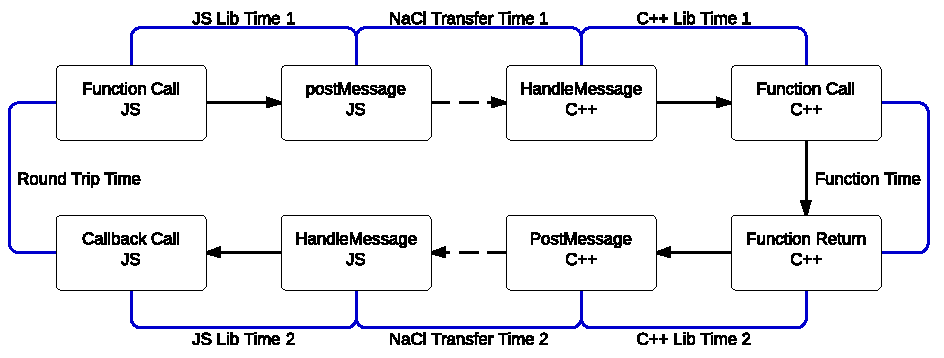
\includegraphics[width=1\textwidth]{RoundTrip.pdf} 
    \caption{A depiction of the round trip time from JavaScript to C++}
    \label{fig:rpc_roundtrip}
\end{figure}


\begin{table}[h]
\centering
\begin{tabular}{l|lll}
\textbf{Type}       & \textbf{Mean RT/s} & \textbf{Uncertainty} & \textbf{Number of runs} \\ \hline
\textbf{long}       & 418                & $\pm$1.79\%              & 56                      \\
\textbf{double}     & 423                & $\pm$2.08\%              & 48                      \\
\textbf{DOMString}  & 420                & $\pm$1.25\%              & 43                      \\
\textbf{dict}       & 415                & $\pm$2.39\%              & 44                      \\
\textbf{nestedDict} & 385                & $\pm$1.29\%              & 47                     
\end{tabular}
\caption{Round trip performance of sending a single parameter}
\label{table:roundtrip_single_param}
\end{table}


\begin{table}[h]
\centering
\begin{tabular}{l|lllll}
\multirow{2}{*}{\textbf{Array Length}} & \multicolumn{5}{l}{\textbf{Round trips per second}}                                        \\
                                       & \textbf{long} & \textbf{double} & \textbf{DOMString} & \textbf{dict} & \textbf{nestedDict} \\ \hline
\textbf{10}                            & 403               & 403                 & 378                    & 317               & 244                     \\
\textbf{45}                            & 379               & 384                 & 309                    & 182               & 112                     \\
\textbf{100}                           & 354               & 347                 & 234                    & 110               & 60.07                   \\
\textbf{450}                           & 237               & 235                 & 102                    & 32.82             & 15.83                   \\
\textbf{1000}                          & 163               & 160                 & 55.41                  & 15.39             & 7.43                    \\
\textbf{4500}                          & 49.39             & 48.93               & 14.60                  & 3.62              & 1.68                    \\
\textbf{10000}                         & 24.68             & 24.50               & 6.62                   & 1.62              & 0.75                    \\
\textbf{45000}                         & 5.99              & 5.98                & 1.28                   & 0.33              & 0.15                   
\end{tabular}
\caption{Round trip performance for arrays of different lengths and types}
\label{table:roundtrip_array}
\end{table}

Tables \ref{table:roundtrip_array} and \ref{table:roundtrip_single_param} show the number of round trips performed in a second for RPC calls with a single parameter and different array lengths. To compare these times, Figure \ref{fig:arraylength-time-plot} shows a column chart visualisation of the data.

\begin{figure}
    \centering
    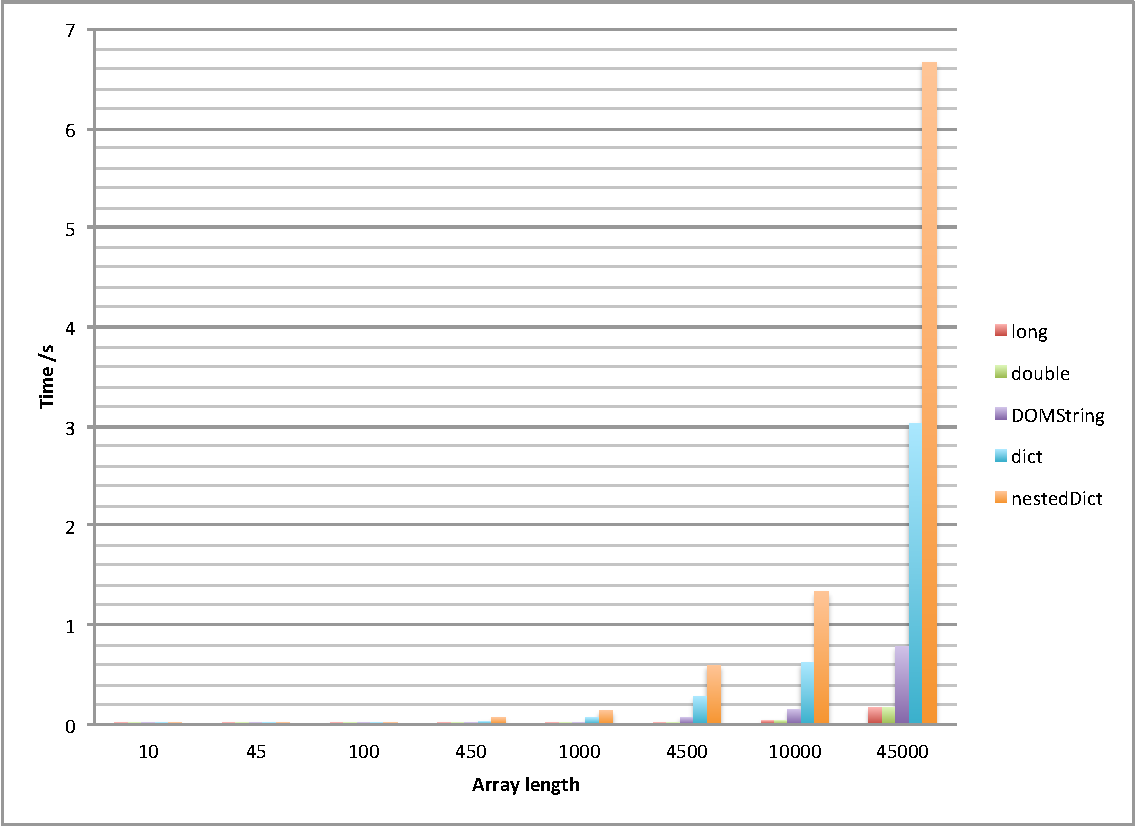
\includegraphics[width=1\textwidth]{arraylength-time-plot.pdf} 
    \caption{The round trip time for arrays of different lengths and types}
    \label{fig:arraylength-time-plot}
\end{figure}


\begin{figure}
    \centering
    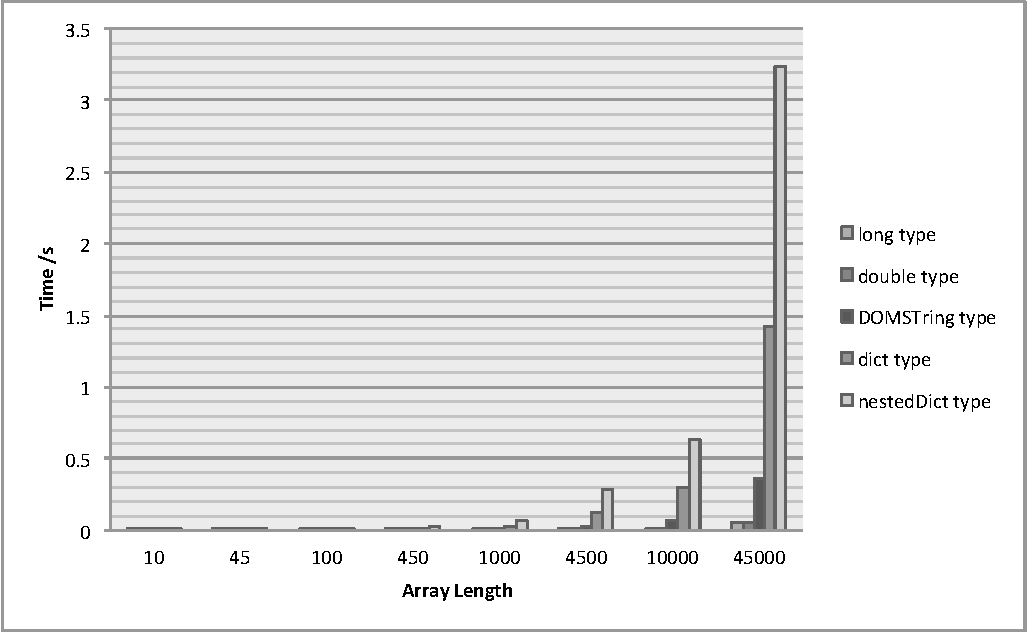
\includegraphics[width=1\textwidth]{arraylength-time-cpp-plot.pdf} 
    \caption{The C++ library time for arrays of different lengths and types}
    \label{fig:arraylength-time-cpp-plot}
\end{figure}



\subsection{C++ Library Time}\label{c-library-time}

We measure the number of microseconds taken to handle a RPC call. This is the time it takes to detect it is an RPC call, extract parameters, convert them, find the method, call it, pack the result, and post the message back to JS.

The results are measured and averaged for the same runs that were performed above. Tables \ref{table:cpp_lib_time_single_param} and \ref{table:cpp_lib_time_arrays} show the results, and Figure \ref{fig:arraylength-time-cpp-plot} shows a visualisation of the data.


\begin{table}[h]
\centering
\begin{tabular}{l|ll}
\textbf{Type}       & \textbf{Mean lib time/$\mu$s} & \textbf{Uncertainty (1 sd)} \\ \hline
\textbf{long}       & 106                       & 18                          \\
\textbf{double}     & 104                       & 17                          \\
\textbf{DOMString}  & 104                       & 18                          \\
\textbf{dict}       & 136                       & 23                          \\
\textbf{nestedDict} & 180                       & 28                         
\end{tabular}
\caption{Mean C++ library time for sending and receiving single parameters of different types}
\label{table:cpp_lib_time_single_param}
\end{table}


\begin{table}[h]
\centering
\begin{tabular}{l|lllll}
\multirow{2}{*}{\textbf{Array Length}} & \multicolumn{5}{l}{\textbf{Time / $\mu$s}}                                                                             \\
                                       & \textbf{long} & \textbf{double} & \textbf{DOMSTring} & \textbf{dict} & \textbf{nestedDict} \\ \hline
\textbf{10}                            & 125                & 126                  & 197                     & 453                & 861                      \\
\textbf{45}                            & 169                & 163                  & 484                     & 1513               & 3273                     \\
\textbf{100}                           & 243                & 246                  & 906                     & 3445               & 7010                     \\
\textbf{450}                           & 705                & 704                  & 3735                    & 13629              & 28198                    \\
\textbf{1000}                          & 1276               & 1355                 & 7607                    & 29582              & 63494                    \\
\textbf{4500}                          & 5548               & 5564                 & 30485                   & 132122             & 292828                   \\
\textbf{10000}                         & 11283              & 11376                & 68444                   & 301438             & 632956                   \\
\textbf{45000}                         & 50532              & 50843                & 359134                  & 1418792            & 3242286                  \\
\textbf{100000}                        & 104087             & 114020               & 799743                  & 3319250            & 7347985                 
\end{tabular}
\caption{Mean C++ library time for sending and receiving arrays of different lengths and types}
\label{table:cpp_lib_time_arrays}
\end{table}

\subsection{JS Library performance}\label{js-library-performance}

The JS library performance \textbf{without} client-side type validation has also been measured, however its performance impact is negligible. The slowest benchmark was found to take approx 3 microseconds (269,253 ops/sec $\pm$  1.90\%).

\subsection{Analysis}\label{analysis}

From the data, we can see that for small types, the most contributing factor to performance is the browser (e.g.~event system, etc.) and PPAPI libraries (how PPAPI implements postMessage). For example, sending a single long type takes 2392.34 microseconds (.002 seconds), but our library only spends 105.5 microseconds processing the call (less than 5\% of the time).

For large and complicated data, the impact of using the library becomes higher and higher. For example, sending 45000 nested objects (which are actually quite simple) has a total round-trip time of 6.67s, and a whole 3.24 seconds of this is spent in our library (i.e.~half the time).

The most likely reason for this is that the C++ library takes O(n) time to process the data in order to marshal it, by converting it from a \lstinline{pp::VarArray} into a \lstinline{std::vector}.

We also notice that the DOMString and Dictionary types are the slowest to marshal and de-marshal. One reason for this could be that number types have a standard representation so perhaps the PPAPI was able to improve how they are transferred, whilst the string types and dictionary types would need marshalling even by the PPAPI. One obvious reason for why the dictionary types take longer to marshal is that they contain multiple types, each type is individually marshalled. So sending a dictionary with multiple keys and values is almost equivalent to sending multiple values separately.

% section performance_evaluation (end)